% Options for packages loaded elsewhere
\PassOptionsToPackage{unicode}{hyperref}
\PassOptionsToPackage{hyphens}{url}
%
\documentclass[
  12pt,
  a4paper,
  twoside]{article}
\usepackage{amsmath,amssymb}
\usepackage{setspace}
\usepackage{iftex}
\ifPDFTeX
  \usepackage[T1]{fontenc}
  \usepackage[utf8]{inputenc}
  \usepackage{textcomp} % provide euro and other symbols
\else % if luatex or xetex
  \usepackage{unicode-math} % this also loads fontspec
  \defaultfontfeatures{Scale=MatchLowercase}
  \defaultfontfeatures[\rmfamily]{Ligatures=TeX,Scale=1}
\fi
\usepackage{lmodern}
\ifPDFTeX\else
  % xetex/luatex font selection
\fi
% Use upquote if available, for straight quotes in verbatim environments
\IfFileExists{upquote.sty}{\usepackage{upquote}}{}
\IfFileExists{microtype.sty}{% use microtype if available
  \usepackage[]{microtype}
  \UseMicrotypeSet[protrusion]{basicmath} % disable protrusion for tt fonts
}{}
\makeatletter
\@ifundefined{KOMAClassName}{% if non-KOMA class
  \IfFileExists{parskip.sty}{%
    \usepackage{parskip}
  }{% else
    \setlength{\parindent}{0pt}
    \setlength{\parskip}{6pt plus 2pt minus 1pt}}
}{% if KOMA class
  \KOMAoptions{parskip=half}}
\makeatother
\usepackage{xcolor}
\usepackage[left=3.9cm, right=3.3cm, top=2.5cm, bottom=3cm]{geometry}
\usepackage{longtable,booktabs,array}
\usepackage{calc} % for calculating minipage widths
% Correct order of tables after \paragraph or \subparagraph
\usepackage{etoolbox}
\makeatletter
\patchcmd\longtable{\par}{\if@noskipsec\mbox{}\fi\par}{}{}
\makeatother
% Allow footnotes in longtable head/foot
\IfFileExists{footnotehyper.sty}{\usepackage{footnotehyper}}{\usepackage{footnote}}
\makesavenoteenv{longtable}
\usepackage{graphicx}
\makeatletter
\def\maxwidth{\ifdim\Gin@nat@width>\linewidth\linewidth\else\Gin@nat@width\fi}
\def\maxheight{\ifdim\Gin@nat@height>\textheight\textheight\else\Gin@nat@height\fi}
\makeatother
% Scale images if necessary, so that they will not overflow the page
% margins by default, and it is still possible to overwrite the defaults
% using explicit options in \includegraphics[width, height, ...]{}
\setkeys{Gin}{width=\maxwidth,height=\maxheight,keepaspectratio}
% Set default figure placement to htbp
\makeatletter
\def\fps@figure{htbp}
\makeatother
\setlength{\emergencystretch}{3em} % prevent overfull lines
\providecommand{\tightlist}{%
  \setlength{\itemsep}{0pt}\setlength{\parskip}{0pt}}
\setcounter{secnumdepth}{5}
% definitions for citeproc citations
\NewDocumentCommand\citeproctext{}{}
\NewDocumentCommand\citeproc{mm}{%
  \begingroup\def\citeproctext{#2}\cite{#1}\endgroup}
\makeatletter
 % allow citations to break across lines
 \let\@cite@ofmt\@firstofone
 % avoid brackets around text for \cite:
 \def\@biblabel#1{}
 \def\@cite#1#2{{#1\if@tempswa , #2\fi}}
\makeatother
\newlength{\cslhangindent}
\setlength{\cslhangindent}{1.5em}
\newlength{\csllabelwidth}
\setlength{\csllabelwidth}{3em}
\newenvironment{CSLReferences}[2] % #1 hanging-indent, #2 entry-spacing
 {\begin{list}{}{%
  \setlength{\itemindent}{0pt}
  \setlength{\leftmargin}{0pt}
  \setlength{\parsep}{0pt}
  % turn on hanging indent if param 1 is 1
  \ifodd #1
   \setlength{\leftmargin}{\cslhangindent}
   \setlength{\itemindent}{-1\cslhangindent}
  \fi
  % set entry spacing
  \setlength{\itemsep}{#2\baselineskip}}}
 {\end{list}}
\usepackage{calc}
\newcommand{\CSLBlock}[1]{\hfill\break\parbox[t]{\linewidth}{\strut\ignorespaces#1\strut}}
\newcommand{\CSLLeftMargin}[1]{\parbox[t]{\csllabelwidth}{\strut#1\strut}}
\newcommand{\CSLRightInline}[1]{\parbox[t]{\linewidth - \csllabelwidth}{\strut#1\strut}}
\newcommand{\CSLIndent}[1]{\hspace{\cslhangindent}#1}
\usepackage{booktabs}
\usepackage{libertine}
\usepackage{libertinust1math}
\usepackage{sourcecodepro}
\usepackage{emptypage}
\renewcommand{\textfraction}{0.05}
\renewcommand{\topfraction}{0.8}
\renewcommand{\bottomfraction}{0.8}
\renewcommand{\floatpagefraction}{0.75}
%\DefineVerbatimEnvironment{Highlighting}{Verbatim}{commandchars=\\\{\},fontsize=\footnotesize}
%% change fontsize of output
\let\oldverbatim\verbatim
\let\endoldverbatim\endverbatim
\renewenvironment{verbatim}{\footnotesize\oldverbatim}{\endoldverbatim}
\ifLuaTeX
  \usepackage{selnolig}  % disable illegal ligatures
\fi
\usepackage{bookmark}
\IfFileExists{xurl.sty}{\usepackage{xurl}}{} % add URL line breaks if available
\urlstyle{same}
\hypersetup{
  pdftitle={Development of a German Instrument for Self-Rated Data Literacy},
  pdfauthor={Leonie Hagitte},
  hidelinks,
  pdfcreator={LaTeX via pandoc}}

\title{Development of a German Instrument for Self-Rated Data Literacy}
\usepackage{etoolbox}
\makeatletter
\providecommand{\subtitle}[1]{% add subtitle to \maketitle
  \apptocmd{\@title}{\par {\large #1 \par}}{}{}
}
\makeatother
\subtitle{An Algorithm-based Approach to Scale Development}
\author{Leonie Hagitte}
\date{2024-07-22}

\begin{document}
\maketitle

{
\setcounter{tocdepth}{2}
\tableofcontents
}
\setstretch{1.2}
\newpage\null\thispagestyle{empty}\newpage

\section*{Abstract}\label{abstract}
\addcontentsline{toc}{section}{Abstract}

The increasing relevance of competent and critical handling of data in society not only makes it possible to record this competence, but also makes self-perception with regard to this competence increasingly clear. Previous approaches consider this competence primarily against the specific background of individual target groups, jobs or roles (\citeproc{ref-Cui2023}{Cui et al., 2023}). In addition, only a few explicitly refer to the general population (\citeproc{ref-Carmi2020}{Carmi et al., 2020}; \citeproc{ref-Cui2023}{Cui et al., 2023}). In view of the various theoretical approaches, there is a need for a uniform definition of data literacy in order to create comparability.
Our aim is therefore to derive a holistic definition based on these approaches and to develop a questionnaire for self-perception of one's own data literacy. To this end, the decisive factors for the construct from previous definitions and operationalizations in various disciplines are brought together. Cognitive interviews are conducted iteratively to create and refine the items. The items are then selected using algorithm-based item selection. The facets of data literacy are comprehensively tested for factorial, discriminant, convergent and congruent incremental validity in order to promote a differentiated understanding of the construct. Construct and criterion validity are tested using correlations and hierarchical regression analyses, while cross-validation checks the robustness of the instrument.
Based on a cross-sectional online questionnaire study, we first examine a representative sample of people from the general population. Limitations arise from the cross-sectional design and the heuristic item reduction, which limit predictions of predictive validity. The heterogeneous nature of the construct makes global instrument development and understanding of all participants difficult.
The self-assessment questionnaire promotes a holistic assessment of competence and its perception for further research, for example by comparing self-assessment and actual performance.

\section*{Acknowledgements}\label{acknowledgements}
\addcontentsline{toc}{section}{Acknowledgements}

I dedicate this thesis to

I want to thank my advisers, Prof.~Martin Schultze, Prof.~Timo Lorenz, and Prof.~Manuel Völkle for their time and patience, and my friends for their resourceful advice:

\newpage\null\thispagestyle{empty}\newpage

\section{Background}\label{background}

In the current digital age characterized by an overwhelming influx especially of online information, it is imperative to accurately distinguish credible, well-substantiated news from various forms of rumors, misinformation, and falsehoods(\citeproc{ref-Koltay2017}{Koltay, 2017}; \citeproc{ref-Leighton2021}{Leighton et al., 2021}; \citeproc{ref-Roetzel2019}{Roetzel, 2019}). Previous research has examined our capacity to assess the trustworthiness of news sources and the subsequent effects on online behaviors, such as information-sharing practices (e.g. \citeproc{ref-Pennycook2021}{Pennycook et al., 2021}; \citeproc{ref-Pennycook2019}{Pennycook \& Rand, 2019}).
Thus, the relevance of data literacy in today's society becomes evident as it serves as a potent tool in navigating the complex data-driven environment(\citeproc{ref-Carmi2020}{Carmi et al., 2020}; e.g.: \citeproc{ref-Cui2023}{Cui et al., 2023}; \citeproc{ref-Leighton2021}{Leighton et al., 2021}; \citeproc{ref-risdale2015}{Ridsdale et al., 2015}). In a world characterized by information overload and rapid technological advancements(\citeproc{ref-Koltay2017}{Koltay, 2017}; \citeproc{ref-Leighton2021}{Leighton et al., 2021}; \citeproc{ref-Roetzel2019}{Roetzel, 2019}), individuals equipped with strong data literacy skills can discern patterns, critically evaluate information, and make informed decisions(e.g. \citeproc{ref-Chen2024}{Chen et al., 2024}; \citeproc{ref-Cui2023}{Cui et al., 2023}).
The exploration of citizens' interaction with media and the cultivation of their agency has traditionally started around concepts such as written literacy, media literacy, information literacy, and digital literacy{[}QUELLE{]}. In more recent discussions, data literacy has been approaching relevance among discussed competencies regarding what is necessary for agency in the current society (\citeproc{ref-Carmi2020}{Carmi et al., 2020}; \citeproc{ref-Leighton2021}{Leighton et al., 2021}). Deficiency in data literacy not only exposes individuals to various risks and harms on personal, social, physical, and financial levels but also constrains their capacity to actively engage as informed citizens within an evolving, data-driven society (\citeproc{ref-Carmi2020}{Carmi et al., 2020}; \citeproc{ref-Leighton2021}{Leighton et al., 2021}). Thus, data literacy is a competency that is becoming increasingly important to everyone. Research has acknowledged this in recent years, as more and more research is being done in that direction (\citeproc{ref-Chen2024}{Chen et al., 2024}; \citeproc{ref-Cui2023}{Cui et al., 2023}). This study aims to complement the current research, with a self rating questionnaire for assessing data literacy among citizens.

Data literacy involves the ability to effectively collect, manage, evaluate, and apply data in a critical manner(\citeproc{ref-risdale2015}{Ridsdale et al., 2015}). According to Wolff et al. (\citeproc{ref-wolff2016}{2016}), it means being able to ask and answer everyday questions using both small and large datasets while considering ethical aspects. This includes skills such as selecting, cleaning, analyzing, visualizing, criticizing, and interpreting data, as well as communicating insights from data and using data for various purposes. Frank (\citeproc{ref-frank2016}{2016}) distinguish between cognitive skills, like data collection and analysis, and social skills, which involve trusting data while maintaining skepticism. Calzada Prado \& Marzal (\citeproc{ref-prado2013}{2013}) outline five dimensions of data literacy: understanding data, acquiring data, interpreting and evaluating data, managing data, and using data. Understanding data includes knowing their types, roles, and significance, while acquiring data involves evaluating and selecting sources. Interpreting and evaluating data encompass understanding different presentation methods and data interpretation. Using data involves preparation, analysis, communication, and ethical considerations. Managing data includes storage, management, and reuse(\citeproc{ref-prado2013}{Calzada Prado \& Marzal, 2013}).
This small comparison already highlights one prominent feature of data literacy - It is a heterogeneous concept(\citeproc{ref-Chen2024}{Chen et al., 2024}). Every subject or profession seems to hold their own definition or framework of data literacy (\citeproc{ref-Chen2024}{Chen et al., 2024}; \citeproc{ref-Cui2023}{Cui et al., 2023}). While that most certainly is good for assessing specific skills (e.g.~in an Recruitment test), it limits the generalisability and comparability of data literacy across individuals with different background. It furthermore limits the accuracy of communication about the topic as two people with different background might hold different definitions on data literacy. In the study from Cui et al. (\citeproc{ref-Cui2023}{2023}) it also becomes apparent, that one group seems to be underrepresented in the research on data literacy: citizens.
Despite being the largest demographic group, citizens are often overlooked in favor of specific professions such as researchers, librarians, students, or educators(\citeproc{ref-Cui2023}{Cui et al., 2023}). Citizens in this case mean people of the general public, that hold no special role or profession, related to data handling or aspects related to data literacy (\citeproc{ref-wolff2016}{Wolff et al., 2016}). This trend raises questions about the emphasis on certain aspects of data literacy, many of which tend to align more closely with professional roles than with the needs of laypeople (\citeproc{ref-schuxfcller2020}{Schüller, 2020}).
In their Framework Schüller (\citeproc{ref-schuxfcller2020}{2020}) highlight the different roles in their data literacy framework: Some of the facets or skills regard ``data-consumption'', whereas the most are skills ``data-producers'' would have. This is also reflected when taking a look into related concepts. The definition proposed by Wolff et al. (\citeproc{ref-wolff2016}{2016}) suggests that data literacy shares some common competencies with statistical and information literacies.

Information literacy, often studied in library sciences, overlaps with data literacy in terms of accessing, critically evaluating, and using data sources (\citeproc{ref-prado2013}{Calzada Prado \& Marzal, 2013}; \citeproc{ref-shields2005}{Shields, 2005}). Wolff et al. (\citeproc{ref-wolff2016}{2016}) also emphasize the importance of the data inquiry process, starting from identifying problems, designing studies, acquiring data, conducting analysis, to drawing data-based conclusions.
In comparison, Gould (\citeproc{ref-gould2017}{2017}) argued that data literacy is essentially the same as statistical literacy but with additional competencies needed due to the increasing importance of data. These added competencies include understanding who collects the data, how and why data is collected, and understanding data privacy and ownership (\citeproc{ref-gould2017}{Gould, 2017}).
However, while statistical literacy focuses on quantitative data and basic statistics, data literacy extends to the ability to understand, access, evaluate, and use arguments and decision-making based on both quantitative and qualitative data (\citeproc{ref-Cui2023}{Cui et al., 2023}).

The name data literacy suggests that one is talking of some form of capability, skill or ability. Whereas in fact data literacy can be seen as more on the side of competences or proficiencies. The distinction lies in the fact, that many behaviors, incorporated in data literacy go beyond the mere question of whether a person is ``able to do it''. It includes the question of ones motivation to do it. This stands in opposition to a former trend, where such literacies were understood cognitively{[}QUELLEN{]}, thus Concerning the mere cognitive predisposition of a person. When talking about data literacy as a competency, the emphasis lies on the possibility to do or to no do something, assuming that one has the ability to do it. Thus data literacy incorporates several abilities but also certain personal predispositions or convictions{[}QUELLE{]}.

When discussing data literacy, it's essential to understand the distinctions between the terms data and information and their relationship to one another.
The concepts of data and information are foundational in various fields, yet their precise definitions and relationships are often subject to interpretation(e.g. \citeproc{ref-Koltay2017}{Koltay, 2017}; \citeproc{ref-Schneider2013}{Schneider, 2013}). In essence, data can be thought of as raw, unprocessed symbols or observations, lacking inherent meaning (\citeproc{ref-shannon1948}{Shannon, 1948}). Information on one hand is characterized by the amount of surprise data evokes in another person(\citeproc{ref-shannon1948}{Shannon, 1948}). Bates (\citeproc{ref-bates2005}{2005}) on the other hand emphasizes that data evolves into information through interpretation and organization, becoming comprehensible and relevant within a specific context or purpose. Does that mean that data is entropy while information stands in opposition to it?\\
Not necessarily. Shannon (\citeproc{ref-shannon1948}{1948}) defines entropy as a measure of uncertainty or disorder in a system. In information theory, entropy is often associated with the amount of unpredictability or randomness in a set of data. However, entropy can also be viewed as a measure of information content within a system(\citeproc{ref-brillouin1953}{Brillouin, 1953}). This perspective suggests that low entropy corresponds to a high concentration of meaningful information. Similarly, the work of Jaynes (\citeproc{ref-jaynes1957}{1957}) highlights the connection between entropy and information, proposing that information can be quantified in terms of the reduction of uncertainty or entropy in a system.
So according to those voices, while data serves as the raw material from which information is derived, it's the reduction of entropy through organization and interpretation that becomes meaningful information. Thus, rather than viewing data as synonymous with entropy or information, it's more accurate to consider information as emerging from the structured representation of data.

It is structured representation of data, that also according to the framework of (\citeproc{ref-schuxfcller2020}{Schüller, 2020}), citizens are primarily concerned with: Citizens holding roles where they mainly consume data or information. Consequently, they may encounter difficulties with tasks or items related to producing facets such as providing or exploiting data. This imbalance could potentially undermine the fairness of tests and questionnaires designed to assess data literacy. Particularly, if these assessments prioritize data and statistical literacy over information literacy. Therefore, our objective was to formulate a definition that adequately addresses both domains, ensuring a balanced representation.

\subsection{Conceptual Integration}\label{conceptual-integration}

Thus, via conceptual integration arrived at the following definition: data literacy is the ability to collect, manage, evaluate, and apply data effectively. It involves asking and answering real-world questions from datasets while considering ethical use. Core skills include selecting, cleaning, analyzing, visualizing, presenting, critiquing, and interpreting data, information and their sources (\citeproc{ref-Cui2023}{Cui et al., 2023}; \citeproc{ref-risdale2015}{Ridsdale et al., 2015}; \citeproc{ref-wolff2016}{Wolff et al., 2016}).
The construct can be structured in five facets (Comprehension,Evaluation, Integration, Communication \& Statistics) that are also very prominent in most definitions in the literature (\citeproc{ref-Cui2023}{Cui et al., 2023}). We further divided them into ``consumer'' facets (Comprehension,Evaluation \& Integration), which are relevant for nearly every person in society, from citizens up. And ``producer'' facets (Communication \& Statistics), which are mainly relevant for people, actively working with data.

\subsubsection{Comprehension}\label{comprehension}

This factor encompasses skills related to understanding and critically evaluating data and information. It involves the ability to comprehend various forms of data presentation, detect inconsistencies, interpret data comprehensively, and identify logical fallacies. Individuals with high scores on this factor demonstrate a strong aptitude for processing and making sense of information across different formats, enabling them to draw accurate conclusions and insights.

\subsubsection{Evaluation}\label{evaluation}

This factor involves skills related to critically evaluating information sources and discerning between facts and opinions. It encompasses the ability to assess the credibility and reliability of information, considering factors such as the reputation of the source and the context in which the information was presented. Individuals scoring high on this factor demonstrate awareness of potential biases or vested interests in information sources.

\subsubsection{Integration}\label{integration}

This factor relates to the ability to integrate data-driven insights into one's worldview and values. It involves actively seeking comprehensive understanding of various topics, engaging with diverse perspectives, and consciously incorporating data-driven insights. Individuals high in this factor adapt their opinions based on new data, prefer evidence-based information, and ensure their values align with reliable data. They engage with information and perspectives that challenge their existing views, showing a willingness to reassess their opinions and positions based on new data.

\subsubsection{Communication}\label{communication}

This factor revolves around the skill to effectively communicate and present data through various means, including visual formats, verbal explanations, and written descriptions.
It requires translating complex data into clear formats, ensuring comprehension by varied audiences. This includes the ability to translate data into simple visualizations, present findings confidently, and articulate complex information effectively in written and visual as well as verbal formats.

\subsubsection{Statistics}\label{statistics}

This factor covers skills related to managing and analyzing data effectively. It involves proficiency in organizing and analyzing data using software tools, conducting statistical analyses, and understanding research methodologies.
As well as conducting interviews or surveys for data collection, performing basic statistical analysis and recognizing trends in graphical representations. Individuals scoring high on this factor exhibit competence in statistical methods, enabling them to effectively analyze data and interpret findings.

\begin{figure}

{\centering 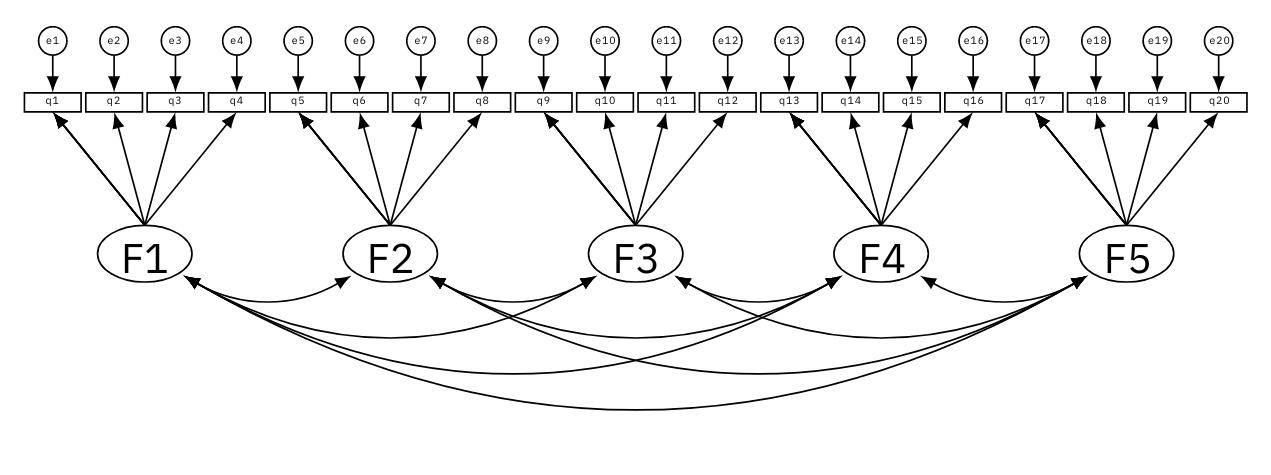
\includegraphics[width=1\linewidth]{images/Models_MA} 

}

\caption{Illustration of the Model data literacy.  }\label{fig:model1}
\end{figure}

\subsection{Delineation from other concepts - Convergent Constructs}\label{delineation-from-other-concepts---convergent-constructs}

This definition of data literacy encompasses certain characteristics and behaviors from similar constructs. Examples for those convergent constructs are: critical thinking, media competency, technology competency, statistical literacy as well as from information literacy(\citeproc{ref-Chen2024}{Chen et al., 2024}; \citeproc{ref-Cui2023}{Cui et al., 2023}; \citeproc{ref-Leighton2021}{Leighton et al., 2021}). As those constructs share substantive parts, differing in size regarding the respective definition of the constructs, it is to be expected that all of them show moderate to strong positive correlations.

Our definition incorporates statistical literacy (\citeproc{ref-Gal2002}{Gal, 2002}) by emphasizing data interpretation, analysis, and understanding different types of data representations, such as graphs and tables (Statistics). It includes elements of information literacy (\citeproc{ref-ACRL2000}{Association of College \& Research Libraries, 2000}) by focusing on evaluating the credibility of data sources, considering factors like reputation and biases, similar to assessing the quality of information sources (Evaluation \& Integration)(\citeproc{ref-Webber2017}{Webber \& Johnston, 2017}). Both statistical and information literacy involve using data and information to make informed decisions (\citeproc{ref-Gal2002}{Gal, 2002}; \citeproc{ref-Webber2017}{Webber \& Johnston, 2017}). Data literacy emphasizes integrating data-driven insights into one's opinions and values, which influence decision-making processes, without focusing on the decision making. Thereby it aligns with the goals of statistical and information literacy. The factor ``Comprehension'' encompasses behaviors and skills associated with critical thinking (\citeproc{ref-payan2022}{Payan Carreira et al., 2022}; \citeproc{ref-rear2019}{Rear, 2019}), such as identifying weaknesses in one's reasoning or actively shaping discourse and public dissemination of information. The factors ``Evaluation'' and ``Statistics'' encompass behaviors and skills related to technology competency, including navigating and critically evaluating online sources and platforms, using information and communication technology, and utilizing statistical software. The ``consumer'' factors are closely related to media literacy, focusing on skills related to critically analyzing and interpreting various media formats for understanding and engaging with media content.\\
In contrast to our definition, statistical literacy often focuses more narrowly on statistical concepts and methods, such as probability, sampling, and hypothesis testing (\citeproc{ref-Gal2002}{Gal, 2002}). Our definition encompasses a broader range of skills beyond statistical concepts, such as data visualization, software usage, and understanding data collection methods. While information literacy involves assessing the quality of information sources, our definition places a particular emphasis on assessing data quality, considering factors like sample size, biases, and data context. This aspect extends beyond traditional information literacy (\citeproc{ref-ACRL2000}{Association of College \& Research Libraries, 2000}) and is more specific to data literacy. Data literacy involves proficiency in using technology, but specifically focuses on understanding and working with data. Technology competency encompasses a broader set of digital skills that extend beyond those relevant for data literacy.

\begin{figure}

{\centering 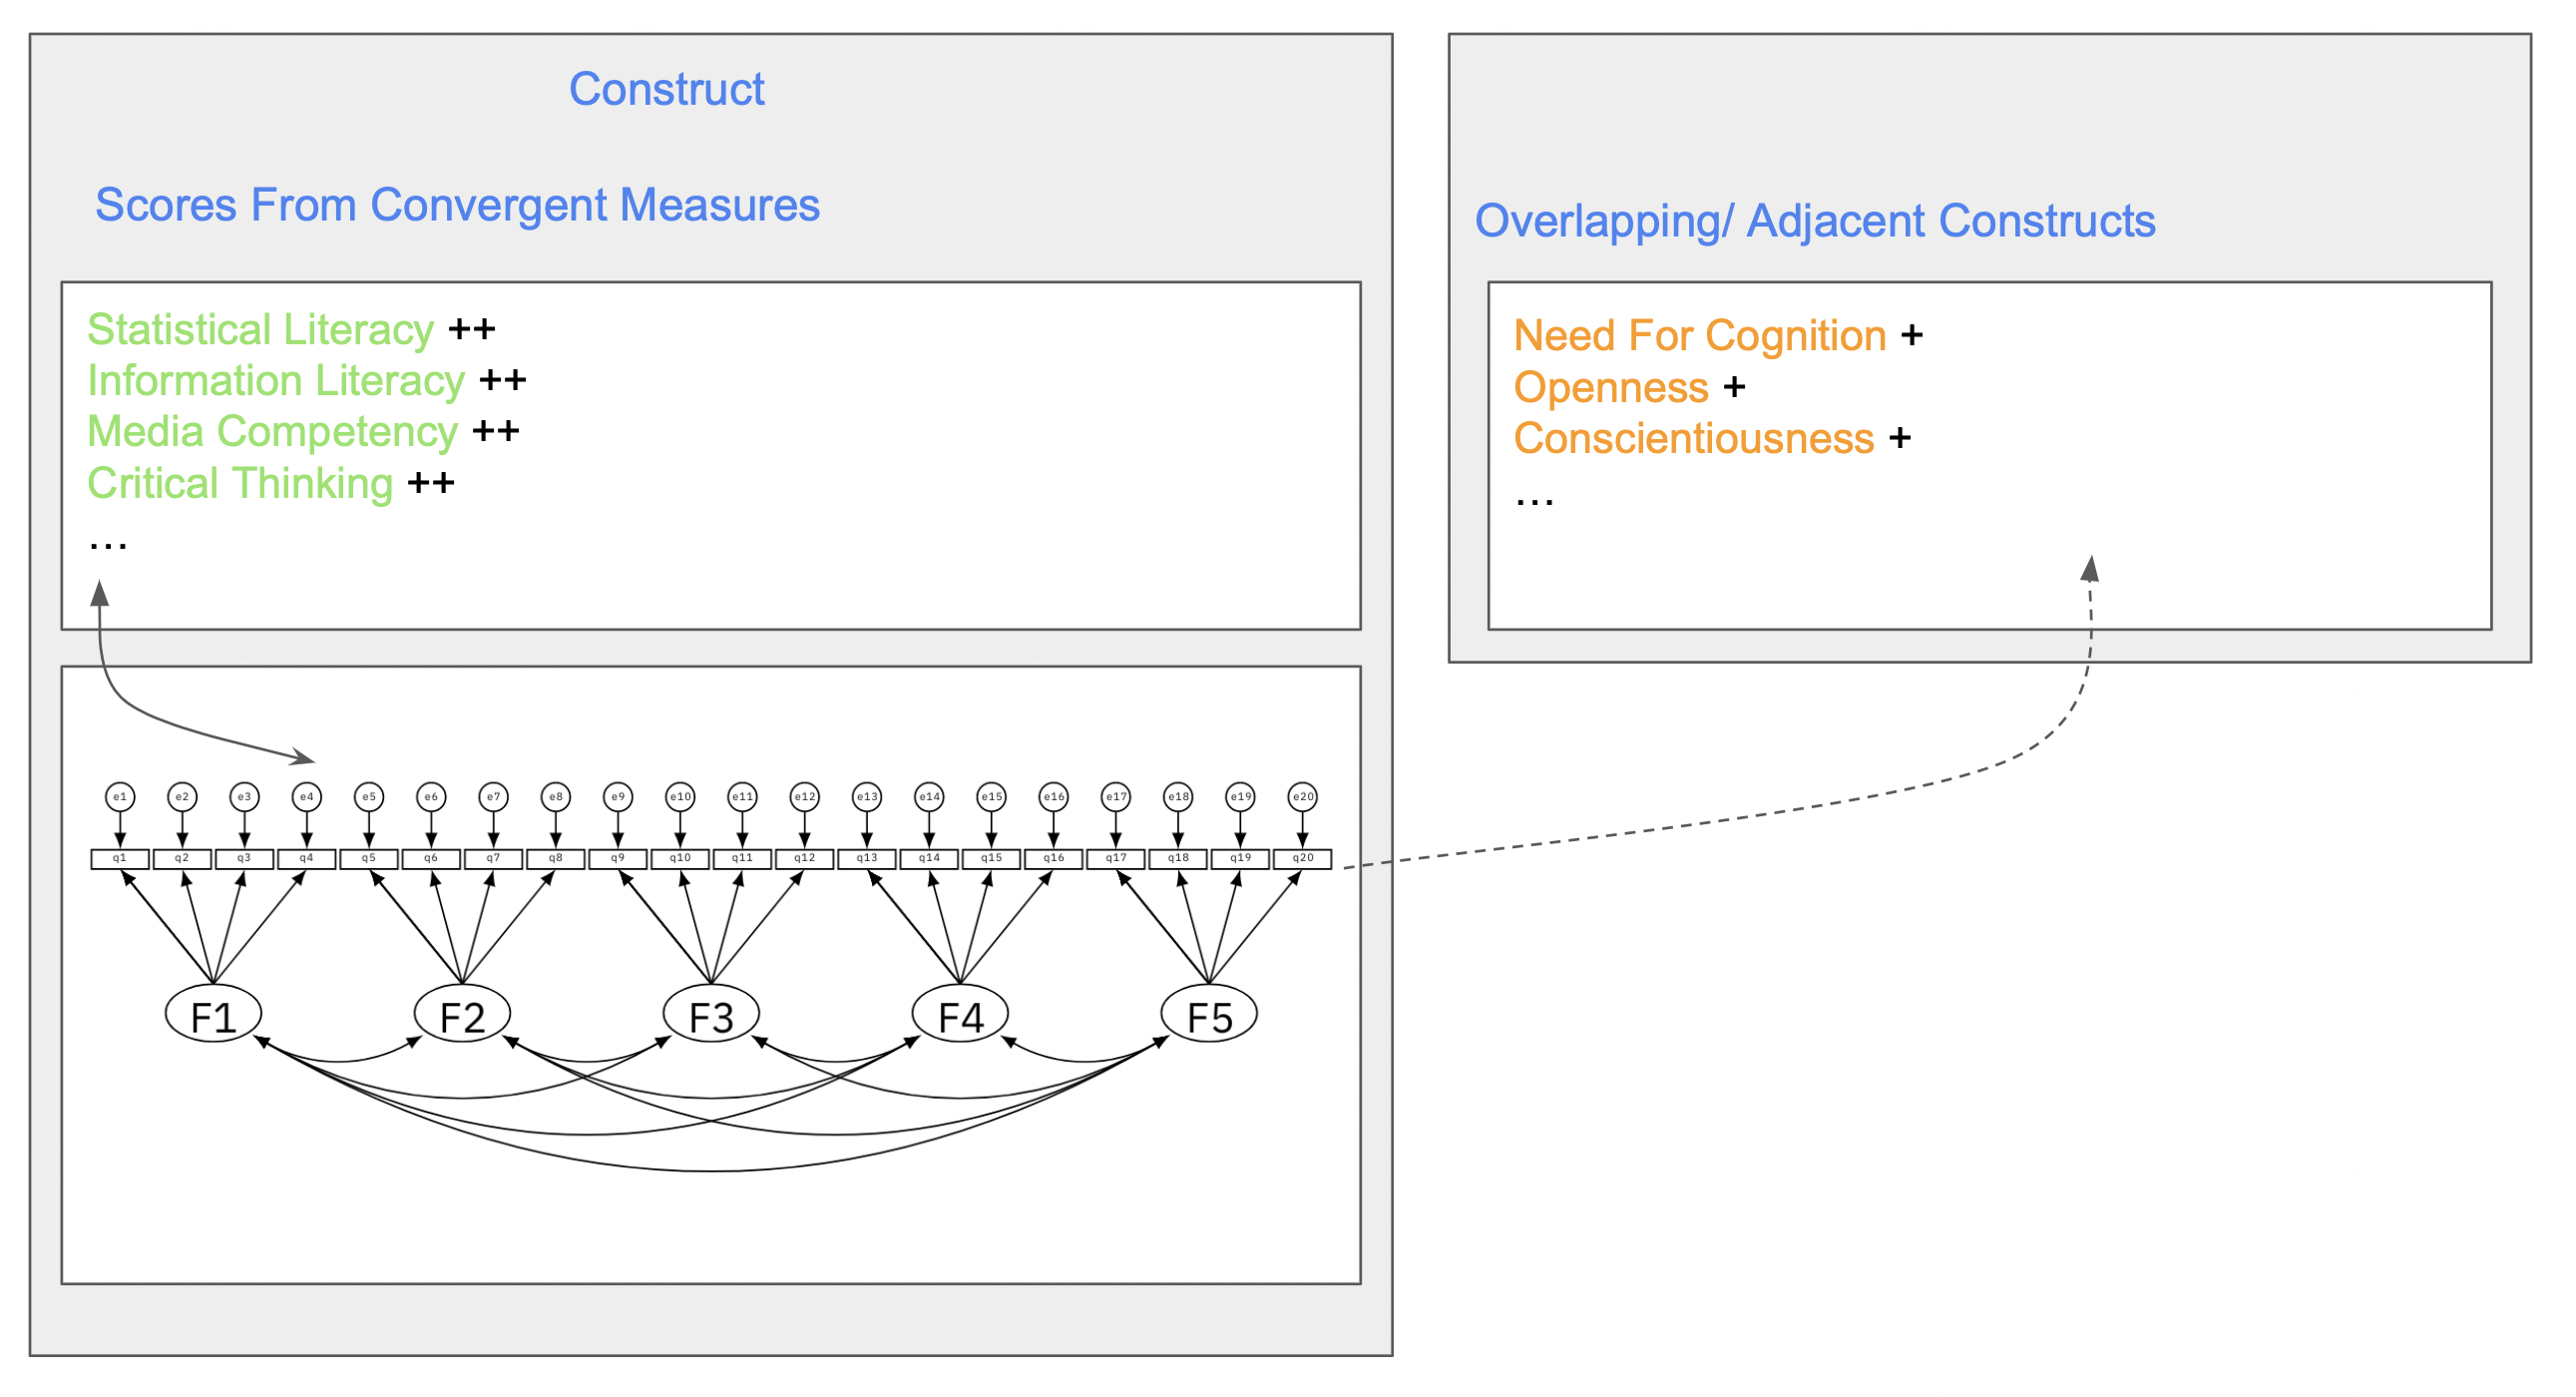
\includegraphics[width=1\linewidth]{images/DL_NomNet} 

}

\caption{Illustration of the nomological net of data literacy.  }\label{fig:nomnet}
\end{figure}

\subsection{Discrimminant Constructs}\label{discrimminant-constructs}

\subsubsection{Need for Cognition}\label{need-for-cognition}

The personality trait known as \emph{Need for Cognition} (NFC) originated in social psychology during the 1940s and 1950s, the concept of NFC, representing an inclination for joyful thinking, is evident in the works of Maslow (\citeproc{ref-maslow1943}{1943}), Murphy (\citeproc{ref-murphy1947}{1947}), Asch (\citeproc{ref-asch1952}{1952}), and Sarnoff \& Katz (\citeproc{ref-sarnoff1954}{1954}). The conceptualization of NFC underwent refinement in the mid-1950s through experimental investigations by Cohen and colleagues (\citeproc{ref-cohen1955}{Cohen et al., 1955}). They defined NFC as ``a need to structure relevant situations in meaningful, integrated ways. It is a need to understand and make reasonable the experiential world'' (\citeproc{ref-cohen1955}{Cohen et al., 1955, p. 291}). The concept captures individual variations in the engagement and enjoyment of thinking tasks (\citeproc{ref-bless1994}{Bless et al., 1994}). As data literacy incorporates several cognitive aspects as well as the motivation to understand data and information one gets presented with, it is expected to correlate positively with ones need for cognition. As need for cognition is more trait like and data literacy is more a competency and therefore less stable, it should not correlate too highly positive, the correlation should be small.

\subsubsection{Opennes to new experiences}\label{opennes-to-new-experiences}

\emph{Openness to new experiences} reflects a broad appreciation for art, emotion, adventure, unconventional ideas, imagination, curiosity, and diverse experiences. Individuals high in openness tend to be intellectually curious, receptive to emotions, appreciative of beauty, and eager to explore new possibilities (Ambridge, 2014). They are often more creative and emotionally attuned compared to those low in openness. However, they may also be perceived as unpredictable and prone to engaging in risky behaviors, including drug use (Ambridge, 2014). High openness is associated with seeking intense and euphoric experiences as a means of self-actualization. In contrast, individuals low in openness tend to seek fulfillment through perseverance and are characterized as pragmatic and data-driven, sometimes viewed as dogmatic or closed-minded. The interpretation and contextualization of the openness factor remain debated, partly due to a lack of biological evidence supporting this trait. Unlike other personality traits, openness has not shown consistent associations with specific brain regions in neuroimaging studies (DeYoung et al., 2010). As already mentioned, data literacy can be thought of as a competency, thus incorporating the individual motivation, leading to a certain behavior. Thus, openness to new experiences is expected to correlate positively with data literacy. As openness to new experiences is more trait like and data literacy is not, the correlation is expected to be small.

\subsubsection{Conscientiousness}\label{conscientiousness}

\emph{Conscientiousness} refers to an individual's propensity for self-discipline, dutifulness, and striving for achievement in alignment with external standards or expectations. It encompasses levels of impulse control, regulation, and goal-directed behavior (Toegel \& Barsoux, 2012; Costa \& McCrae, 1992). High conscientiousness is characterized by persistence and focus, often perceived as stubbornness, whereas low conscientiousness is linked to flexibility and spontaneity, potentially manifesting as carelessness and unreliability (Toegel \& Barsoux, 2012). Individuals with high conscientiousness tend to prefer planned actions over spontaneous ones (Costa \& McCrae, 1992).\\
The cognitive aspects of data literacy as well as the motivation to understand data and information speaks to the conscientiousness of people as well. As being critical and at times detail oriented (e.g.~in interpreting results, or spotting inconsistencies in presented information or while examining the credibility of sources) is also integral to data literacy, data literacy and conscientiousness are expected to correlate positively. As conscientiousness also trait opposing to data literacy, they should not correlate to highly positive, the correlation should be small.

\subsection{Aim of the Study}\label{aim-of-the-study}

The aim was to derive a comprehensive definition of data literacy based on existing approaches and to develop a questionnaire for self-rated data literacy with citizens being the target population. An emphasis lies on measuring the three consumer factors of the construct (Comprehension,Evaluation \& Integration). Thus the research question of this study is:

``Does the proposed set of items effectively capture the latent factor structure of self-rated data literacy, and can the created scale be considered a reliable and valid measure of this construct?''

\emph{H1: The test-data will support the suggested latent factor structure and the proposed measurement model.}\\
\emph{H2: The latent factor structure of the initial analysis will be supported by a different sample.}\\
\emph{H3: A moderate to high positive correlation with the SWE-IV-16 (Behm, 2018) is expected.}\\
\emph{H4: A moderate positive correlation with the the ICT-SC25 (Schauffel et al., 2021) is expected.}\\
\emph{H5: A small positive correlation with the NFC-K (Beißert et al., 2015) is expected.}\\
\emph{H6: A small positive correlation with the the BFI-10 (Rammstedt et al., 2014) is expected.}

\section{Methods}\label{methods}

\subsection{Item Creation}\label{item-creation}

A literature review was done to create items and then ten cognitive interviews were held to refine those potential items. The interviews were administered iteratively to refine the items every time a bit more. We will treat the first 25 participants like a pilot, to check for potential problems in the survey.

\subsection{Rationale for Measurement Model}\label{rationale-for-measurement-model}

One decision that needs to be done by the researcher before the item selection with `stuart', is the design of the measurement model, or how many items per factor the final scale should have.
This scale will be created as parsimonious as possible, while ensuring that there is a real model fit to be estimated. So the decision in this case was of statistical nature, while with three items per factor, the model would have been just identified, four items per factor is the most parsimonious choice, where there is already a real model fit, that can be assessed in the end.

\subsection{Sample}\label{sample}

The participants are recruited through a combination of personal and professional networks, along with outreach on several online social media platforms (e.g.~Instagram, LinkedIn, Whatsapp, Telegram and via e-mail) Conducted in German, the participation in the study was entirely voluntary, with no external incentives provided. We conducted a-priori power analysis to determine the necessary sample size for the structural equation modelling. We used the `semPower' package in R (Moshagen \& Bader, 2023) and also took a look into studies with similar goals and methods. The power analysis gave an analytical estimate for N=645, and a simulated estimate N=613, for the respective measurement model. In the literature sample sizes of N=500 up to N=1000 could be found (Algner \& Lorenz, 2022; Remmert et al.,2022; Schneider et al.,2024). So the optimal sample size, we are aiming at, lies somewhere between those numbers.

Participants had to be of legal age, to be included in the study. Furthermore, attention check questions are included (three instructed response items and one seriousness check item, at the end) within the survey to assess participants' attentiveness. Participants who fail to correctly answer two out of the four attention check questions will be excluded from the analysis.

The following characteristics of this studys sample will be made with referral to the respective stat in the German population of 2022.
The sample for this study comprised N=612 participants. Within the sample, 48,3\% identified as female(50,65\%), 50,2\% as male(49,35\%), and 1,5\% did not identify with binary gender categories (\citeproc{ref-StBA2024a}{Statistisches Bundesamt, 2024b}). The average age was XX(M = 44,6)(\citeproc{ref-StBA2024b}{Statistisches Bundesamt, 2024a}), with an average age of XX amongst women (M = 45,9)(\citeproc{ref-StBA2023a}{Statistisches Bundesamt, 2023a}) and XX amongst men (M = 43,2)(\citeproc{ref-StBA2023a}{Statistisches Bundesamt, 2023a}). Regarding education, participants exhibited a {[}insert educational level- specifying the range or types of educational levels observed in the sample{]}. XX\% of the participants had a full time employment at the time(65,15\%; Men = 42,40\%, Women = 22,75\%)(\citeproc{ref-BfA2024}{Bundesargentur für Arbeit, 2024}; \citeproc{ref-StBA2023b}{Statistisches Bundesamt, 2023b}), XX\% had an part time employment (28,22\%; Men = 6,16\%; Women = 22,06\%)(\citeproc{ref-BfA2024}{Bundesargentur für Arbeit, 2024}; \citeproc{ref-StBA2023b}{Statistisches Bundesamt, 2023b}) and XX\% had no work at the time of the survey (6,63\%)(\citeproc{ref-BfA2024}{Bundesargentur für Arbeit, 2024}). The study encompassed every sector within the occupational classification at least once (\citeproc{ref-BfA2024}{Bundesargentur für Arbeit, 2024}). XX\% of the participants indicated that they were students at the time of the survey (3,39\%){[}StBA2024c{]}.

\subsection{Open Science Standards}\label{open-science-standards}

This project uses the reproducibility workflow proposed by Peikert et al. (\citeproc{ref-Peikert2021}{2021}). Docker and renv work together to create a reproducible and portable environment. Docker captures the complete software stack, while renv focuses on
managing R package dependencies and providing a clear documentation of the R
package environment. This combination ensures that your analysis can be easily
reproduced and shared with others in a reliable and transparent manner.
The study was preregistered at Zenodo (\url{DOI:10.5281/zenodo.11196495}).

\subsection{Procedure}\label{procedure}

A cross-sectional online survey is used to examine a sample from the general population. Participants complete the Self-perceived Data Literacy Scale alongside demographic questions and additional validation measures. Survey questions of each measurement are randomized for each participant to minimize order effects and response biases. To shorten the overall length of the assessment the questions in each factor of the data literacy questionnaire are randomly selected for each participant. That way each participant only answers half of the possible items, the other half are planned missings.

\subsection{Instruments}\label{instruments}

\subsubsection{Measuring Data Literacy}\label{measuring-data-literacy}

On Data Literacy the participants will be asked to answer 71
items. Each participant will answer 38 items of the 71, that are randomly selected.
To answer the items, respondents indicate their agreement on a five-point Likert
scale (1 = ``strongly disagree'', 2 = ``somewhat disagree'', 3 = ``neither agree nor
disagree'', 4 = ``somewhat agree'', 5 = ``strongly agree'') with a ``don't know''
option.

\subsubsection{Measuring Information Literacy}\label{measuring-information-literacy}

The SWE-IV-16 (Behm, 2018)(McDonalds \(\omega\) = .91; Cronbachs McDonalds \(\alpha\) =.91) assesses the self-efficacy beliefs
of adolescents and adults in their ability to engage in information behaviour. This
questionnaire measures the process model of information-related problem-solving
(Brand-Gruwel et al., 2009). In this study this construct is used as a proxy for information literacy.
It consists of 16 statements addressing self-assessed
abilities in searching for and evaluating information, as well as managing
information searches effectively. Each statement begins with ``When I search for
information on a topic or a specific question\ldots{}'' and respondents indicate their
agreement on a five-point Likert scale (1 = ``strongly disagree'', 2 = ``somewhat
disagree'', 3 = ``neither agree nor disagree'', 4 = ``somewhat agree'', 5 = ``strongly
agree''). The total scale value is computed as the arithmetic
mean of the items, which may be inverted if necessary. Calculation of the total value
requires valid responses to at least 12 of the 16 items. I expect the final questionnaire to correlate moderately up to highly positive with the SWE-IV-16 (Behm, 2018), measuring peoples ability to engage in information behaviour.

\subsubsection{Measuring Need for Cognition}\label{measuring-need-for-cognition}

The NFC-K (Beißert et al., 2015)(McDonalds \(\omega\) = .62; Cronbachs McDonalds \(\alpha\) =.60) is a tool used to assess the
NFC through four items, which represent two facets: ``engagement'' and ``joy''. The
NFC-K is measured with a seven-point response scale, ranging from ``strongly
disagree'' (1) to ``strongly agree'' (7), with a ``neither'' option in the middle. The
German version of the scale is adapted from the original English scale by Cacioppo
and Petty (1982) and translated by Bless et al.~(1994). To determine an individual's NFC score, a mean value
(scale value) is computed from the four raw score points of the responses. The
resulting mean values range between 1 and 7. I expect a small to moderate positive correlation with the NFC-K (Beißert et al., 2015), assessing the Need for Cognition (NFC).

\subsubsection{Measuring Technology Competency}\label{measuring-technology-competency}

To assess self-perceived competence in using information and
communication technology (ICT), the five general items of the ICT-SC25 (Schauffel
et al., 2021) will be used (McDonalds \(\omega\) = .93; Cronbachs McDonalds \(\alpha\) =.93). The ICT-SC25 is a scale consisting of 25 items designed to
assess self-perceived competence in using information and communication
technology. It is available in both German (ICT-SC25g) and English (ICT-SC25e). The
scale measures general and domain-specific ICT competence, including
communication, processing and storing, content generation, safe application, and
problem-solving skills. Items are measured using a six-point fully-labeled Likert-type
rating scale ranging from strongly disagree (1) to strongly agree (6). Researchers can choose to
utilise either the entire scale or individual subscales based on their specific research objectives. The ICT-SC25g/e
is applicable for both manifest and latent analysis. Manifest scale scores for the ICT-
SC25g/e are calculated separately for each subscale by computing the unweighted
mean score of the items within each subscale (Schauffel et al., 2021). I expect a moderate, positive correlation of the final scale with the five general items of the ICT-SC25 (Schauffel et al., 2021).

\subsubsection{Measuring Openness and Conscientiousness}\label{measuring-openness-and-conscientiousness}

The BFI-10 (Rammstedt et al., 2014) will be used to assess
personality based on the five-factor model. Only the items on openness and
conscientiousness were assessed.
The items are answered on a five-point rating scale from ``strongly disagree'' (1) to
``strongly agree'' (5). To measure the respondent's individual traits on the five
personality dimensions, the responses to the two items for each dimension are
averaged. First, the negatively worded item is recoded (items 1, 3, 4, 5, and 7), then
the mean value is calculated for each dimension from both the recoded and non-
recoded items. The values for the five dimensions range from 1 to 5 (see
Rammstedt, 2007 for reference values). I expect small to moderate positive correlations with openness and conscientiousness of the BFI-10 (Rammstedt et al., 2014).

\section{Analysis}\label{analysis}

\subsection{Data Quality}\label{data-quality}

Careless or inattentive response patterns were analyzed by the ATC items. Furthermore, the data was checked for outliers. Because of the planned random missings in the data, those NAs were imputed via the `mice' package, with predictice mean matching. Also for model estimation full information maximum likelihood was used to handle the missing data.

\subsection{Meta-Heuristics}\label{meta-heuristics}

Algorithm-based item selection is used to choose the most relevant items, reducing the initial item pool. In classical approaches items are evaluated within the overall item pool and are then often selected based on their individual properties (e.g.~difficulty, discrimination, item-scale-correlations).
Compared to classical approaches, algorithms are more objective and efficient in finding a good or nearly perfect solution with regard to certain crteria (Leite et~al., 2008; Olaru et~al., 2015). Furthermore, some empirical studies suggest that the use of algorithms leads to similar or better results in scale construction than traditional approaches (Sandyet~al., 2014; Schroeders et~al., 2016; Olaru and Danner, 2021). The automated approach takes the opposite perspective to the classical approach, the one of meta heuristics, by repeatedly estimating CFAs for a multitude of possible item-combinations{[}QUELLE{]}. Thus, a pool of items with some constraints and the goal to find the one combination that best fits the suggested purpose of the final scale is estimated{[}QUELLE{]}.Thus, the selection of items and construction of a questionnaire can be viewed as a combinatorial problem, like the knapsack problem (``Choose a set of objects, each having aspecific weight and monetary value, so that the value is maximized and the total weight does not exceed a predetermined limit;''Schroeders et al., 2016, p.~4; Kerber et~al., 2022).

`Stuart' can construct subsets from a pool of items by using ant-colony- optimization, genetic algorithms, brute force, or random sampling (Schultze, 2022). Those meta-heuristics like are utilized to handle these combinatorial optimization problems.

\begin{center}
$\Phi = F(\textrm{RMSEA}) + F(CFI)+ F(\textrm{SRMR}) + F(\omega) + F(\nu)$
\end{center}

For this study, a set of 20 items from a set of 71 items should be selected, to form a questionnaire. I want to optimize the data literacy self rating scale for model fit criteria and composite reliability (RMSEA, SRMR, CFI \& McDonalds \(\omega\)) as well as variability in the difficulty of items. Those criteria will be defined in the objective function in `stuart' (Schultze, 2020).

\begin{center}
$\Phi = \frac{1}{1 + \exp(-10 \cdot (\omega - 0.6))} + 0.5 \cdot \left(1 - \frac{1}{1 + \exp(-100 \cdot (\textrm{RMSEA} - 0.05))}\right) + 0.5 \cdot \left(1 - \frac{1}{1 + \exp(-100 \cdot (\textrm{SRMR} - 0.06))}\right) - (\textrm{sd}(\nu) - 1.62)^2 + 1.62^2 + 10^{-6}$
\end{center}

I use the genetic algorithm of `stuart' for this. Genetic algorithms are based on Darwinian evolution principles -- selection, crossover, mutation and survival of the fittest(Holland, 1992; Schroeders et~al.,2016). With the genetic algorithm, the initial set of 71 items is to be reduced based on the evolutionary process of selection, but opposing to evolution with a goal: A near-optimal ``solution''. The survival of an item is determined by its quality (called ``fitness'';Galán et~al., 2013). The algorithm is build on two processes: Variation(i.e.~recombination and mutation) and selection. Variation rewards diversity an innovation of items, whereas selection rewards quality or fitness. The algorithm links ``genes'' (i.e.~items), that represent a certain variable, to a ``chromosome'' (i.e.~a set of items). A predefined number of chromosomes are randomly generated from the 1st generation (i.e.~the original item pool). The algorithm tries to maximize the psychometric quality of the ``chromosomes''( i.e.~item sets) by evaluating the ``chromosomes''( i.e.~item sets) against a ``fitness''function. Based on this fitness function, the fittest ``chromosomes''(i.e.~item sets) of each generation are determined, which then form the basis for the next generation (forming the selection process). The process of variation establishes genetic diversity and mutation within the generations by spontaneously exchanging items within a scale or between two scales. This adds a degree of randomness to the selection process. This is done a predefined number of iterations. This way the fittest ``chromosome''(i.e.~set of items), with the highest quality, is to be identified (Schroeders et~al., 2016).

\subsection{Validation}\label{validation}

The provided sample will be divided into two subsets (i.e.~training data and test data) using the `holdout' function in `stuart'. The specified item-selection procedure will be applied to the training data. The training data is undergoing k-fold cross validation (k=3), using the `kfold' function in `stuart'. The other sample, the test data, is used for evaluation of the final models performance, as well as the latent correlations with the convergent measures.
Validation with the test data will be conducted (using the `crossvalidate' function in `stuart') to assess the invariance of the measurement models between the training and testing datasets. Invariance levels will be measured with the `max.invariance' function. Invariance will be necessary to claim that the scale validation has worked.

\section{Results}\label{results}

\subsection{Demographic Results}\label{demographic-results}

On average, participants were working (M/SD). On average, participants were studying (M/SD). Descriptives and Correlations
Table XX
presents descriptive statistics, McDonald's \(\omega\) ,
Cronbach's \(\alpha\) and the correlation matrix for the respective variables.\\
The data literacy scale correlated XXX with the SWE-IV-16(r = , p ). The data literacy scale correlated XXX with the NFC-K(r = , p ). The data literacy scale correlated XXX with the the general items of the ICT-SC25(r = , p ). The data literacy scale correlated XXX with the openness of the BFI-10(r = , p ). The data literacy scale correlated XXX with conscientiousness of the BFI-10(r = , p ). The xxx correlations (r = , p ) between the newly created scale and the SWE-IV-16, NFC-K, the general items of the ICT-SC25 and openness and conscientiousness of the BFI-10,respectively, indicate the data literacy scale measures \#a similar, yet distinct concept\#.

\subsection{Model Fit and Latent Structure in the Construction Sample}\label{model-fit-and-latent-structure-in-the-construction-sample}

The Algorithm selected 20 of the 71 original items representing the five factors Comprehension, Evaluation, Integration, Communication and Statistics with four items each (Figure X). The final solution exhibits good model fit with Satorra-Bentler-\(X^{2}\) (XXX, N = XXX) = XXX, p = XXX,CFI = XXX, TLI = XXX, SRMR = XXX, RMSEA = XXX, 90\%-CIRMSEA {[}XXX; XXX{]}.
Standardized loadings of the factor Comprehension ranged from 0.XX to 0.XX. For the factor Evaluation loadings ranged from 0.XX to 0.XX. For the factor Integration loadings ranged from 0.XX to 0.XX. For the factor Communication loadings ranged from 0.XX to 0.XX. For the factor Statistics loadings ranged from 0.XX to 0.XX.
All factor loadings including standard errors can be found in the Supplementary Material.

\subsection{Model Fit and Latent Structure in the Validation Sample}\label{model-fit-and-latent-structure-in-the-validation-sample}

Cross-validation with the second half of the data indicated that the assumption of XXXX measurement invariance holds across the XXX subsamples: \(X^{2}\)(XXX) = XXX, p \textless{} XXX, CFI = 0.XXX, SRMR = 0.XXX, RMSEA = 0.XXX; \(X^{2}\) = XXX, df = XX, p = 0.XXXX.

residuals
correlates or the residuals for the adjacent constructs

\section{Discussion}\label{discussion}

\subsection{Summarising the results}\label{summarising-the-results}

Everything worked - what do I need to report?
First, report on the three core decisions and how the solution was created, whether it is stable, and how it was validated. The final variant is then reported exactly like a CFA (e.g.~Jackson et al., 2009). To have a clear structure, answer the following questions:
How large was the original item pool and how was it created?
What is the structure of the scale?
Which algorithm was used (or bruteforce)?
Which objective function was used?
How stable is the final variant?
How was the final variant further validated (e.g.~crossvalidate, k-fold)?

\subsection{What does it all mean / ``Why?''}\label{what-does-it-all-mean-why}

\begin{itemize}
\tightlist
\item
  Start with the research question

  \begin{itemize}
  \tightlist
  \item
    Maybe then towards the hypotheses
  \end{itemize}
\item
  connecting findings to the related theories
\item
  very related/ current literature first, than broader is possible
\item
  When discussing the why - be careful, because you didnt test that
\end{itemize}

\subsection{Limitations}\label{limitations}

\begin{itemize}
\tightlist
\item
  sample
\item
  content validity
\item
  DIF?
\item
  psych science - authors guide to generelizability
\item
  attempts to control for limitating factors
\item
  dont include to general/ broad critiques, but special one for my own study
\end{itemize}

This study's results should be interpreted with the following limitations in mind.
As shown in the demographic variables, the sample of this study deviated from the
general public in several points. Thus, this study might not have reached a representative sample
and therefore lack generalizability. Also it is to be kept in mind that this influences the
item pool selected, because this is specifically trained on the sample of this study.
Furthermore the training data set and the testing data set are of different size, which
can influence the MI testing (Chen,2007). Additionally, the sample sizes, although appropriate, ideally could have been larger and are on the lower threshold of the prior poweranalysis (e.g., Kass andTinsley, 1979; Hu and Bentler, 1999).
Although the questionnaire exhibited good model fit, it is to be kept in mind
that algorithm based item selection is essentially a heuristic approach and does not
always result in the best solution there is.

\subsection{Future directions}\label{future-directions}

Construct validity is evaluated through confirmatory factor analysis (CFA), using MLR as estimator, as well as correlation analyses with related constructs

\begin{itemize}
\tightlist
\item
  what to optimize the scale for?
\item
  dynamic fit indices
\item
  factors 4 and 5

  \begin{itemize}
  \tightlist
  \item
    adaptive testing/ IRT

    \begin{itemize}
    \tightlist
    \item
      dimensionality assumption and computationally intense
    \end{itemize}
  \item
    CART - tree based adaptive testing (classification trees) always binary split

    \begin{itemize}
    \tightlist
    \item
      gini index to identify the cut off
    \item
      POMP method - for differing number of answer formats
    \end{itemize}
  \end{itemize}
\item
  residuals correlates
\item
  heterogeneity of construct
\end{itemize}

The heterogeneous nature of the construct complicates global instrument development and understanding across all participants. The measure is designed for citizens, potentially limiting discrimination at higher item difficulties or among more literate participants, a direction we aim to improve in future studies.

Noteworthy is the inherent approximate, rather than deterministic, nature of metaheuristics (Schultze \& Lorenz ,2023; Blum and Roli, 2003).

\section*{References}\label{references}
\addcontentsline{toc}{section}{References}

\phantomsection\label{refs}
\begin{CSLReferences}{1}{0}
\bibitem[\citeproctext]{ref-asch1952}
Asch, S. (1952). \emph{Social psychology}. Prentice Hall.

\bibitem[\citeproctext]{ref-ACRL2000}
Association of College \& Research Libraries. (2000). \emph{Information literacy competency standards for higher education}. Brochure; American Library Association.

\bibitem[\citeproctext]{ref-bates2005}
Bates, M. J. (2005). An introduction to metatheories, theories, and models. In M. J. Bates \& M. N. Maack (Eds.), \emph{Encyclopedia of library and information sciences} (2nd ed., pp. 109--121). Taylor \& Francis.

\bibitem[\citeproctext]{ref-bless1994}
Bless, H., Wänke, M., Bohner, G., Fellhauer, R., \& Schwarz, N. (1994). Need for cognition: Eine skala zur erfassung von engagement und freude bei denkaufgaben {[}presentation and validation of a german version of the need for cognition scale{]}. \emph{Zeitschrift Für Sozialpsychologie}, \emph{25}, 147--154.

\bibitem[\citeproctext]{ref-brillouin1953}
Brillouin, L. (1953). Negentropy principle of information. \emph{Journal of Applied Physics}, \emph{24}(9), 1152--1163.

\bibitem[\citeproctext]{ref-BfA2024}
Bundesargentur für Arbeit. (2024). \emph{Arbeitslosenzahl in deutschland im jahresdurchschnitt von 2005 bis 2024}. \url{https://de.statista.com/statistik/daten/studie/1223/umfrage/arbeitslosenzahl-in-deutschland-jahresdurchschnittswerte/\#:~:text=Im\%20Monat\%20Juni\%202024\%20waren,um\%20rund\%20178.800\%20Personen\%20höher}; Statista.

\bibitem[\citeproctext]{ref-prado2013}
Calzada Prado, J., \& Marzal, M. Á. (2013). Incorporating data literacy into information literacy programs: Core competencies and contents. \emph{Libri}, \emph{63}(2), 123--134. \url{https://doi.org/10.1515/libri-2013-0010}

\bibitem[\citeproctext]{ref-Carmi2020}
Carmi, E., Yates, S. J., Lockley, E., \& Pawluczuk, A. (2020). Data citizenship: Rethinking data literacy in the age of disinformation, misinformation, and malinformation. \emph{Internet Policy Review}, \emph{9}(2). \url{https://doi.org/10.14763/2020.2.1481}

\bibitem[\citeproctext]{ref-Chen2024}
Chen, F., Cui, Y., Lutsyk-King, A., Gao, Y., Liu, X., Cutumisu, M., \& Leighton, J. P. (2024). Validating a novel digital performance-based assessment of data literacy: Psychometric and eye-tracking analyses. \emph{Education and Information Technologies}, \emph{29}(8), 9417--9444. \url{https://doi.org/10.1007/s10639-023-12177-7}

\bibitem[\citeproctext]{ref-cohen1955}
Cohen, A. R., Stotland, E., \& Wolfe, D. M. (1955). An experimental investigation of need for cognition. \emph{The Journal of Abnormal and Social Psychology}, \emph{51}(2), 291--294. \url{https://doi.org/10.1037/h0042761}

\bibitem[\citeproctext]{ref-Cui2023}
Cui, Y., Chen, F., Lutsyk, A., Leighton, J., \& Cutumisu, M. (2023). Data literacy assessments: A systematic literature review. \emph{Assessment in Education: Principles, Policy \& Practice}, \emph{30}, 1--21. \url{https://doi.org/10.1080/0969594X.2023.2182737}

\bibitem[\citeproctext]{ref-frank2016}
Frank, M. (2016). Data literacy - what is it and how can we make it happen? \emph{Journal of Community Informatics}, \emph{12}, 4--8.

\bibitem[\citeproctext]{ref-Gal2002}
Gal, I. (2002). Adults' statistical literacy: Meanings, components, responsibilities. \emph{International Statistical Review / Revue Internationale de Statistique}, \emph{70}(1), 1--25. \url{http://www.jstor.org/stable/1403713}

\bibitem[\citeproctext]{ref-gould2017}
Gould, R. (2017). Data literacy is statistical literacy. \emph{Statistics Education Research Journal}, \emph{16}(1), 22--25. \url{https://doi.org/10.52041/serj.v16i1.209}

\bibitem[\citeproctext]{ref-jaynes1957}
Jaynes, E. T. (1957). Information theory and statistical mechanics. \emph{Physical Review}, \emph{106}(4), 620--630.

\bibitem[\citeproctext]{ref-Koltay2017}
Koltay, T. (2017). Information overload in a data-intensive world. In A. J. Schuster (Ed.), \emph{Understanding information: From the big bang to big data} (pp. 197--217). Springer International Publishing. \url{https://doi.org/10.1007/978-3-319-59090-5_10}

\bibitem[\citeproctext]{ref-Leighton2021}
Leighton, J. P., Cui, Y., \& Cutumisu, M. (2021). Key information processes for thinking critically in data-rich environments. \emph{Frontiers in Education}, \emph{6}. \url{https://doi.org/10.3389/feduc.2021.561847}

\bibitem[\citeproctext]{ref-maslow1943}
Maslow, A. H. (1943). A theory of human motivation. \emph{Psychological Review}, \emph{50}(4), 370--396. \url{https://doi.org/10.1037/h0054346}

\bibitem[\citeproctext]{ref-murphy1947}
Murphy, G. (1947). \emph{Personality: A biosocial approach to origins and structure}. Harper.

\bibitem[\citeproctext]{ref-payan2022}
Payan Carreira, R., Sacau-Fontenla, A., Rebelo, H., Sebastião, L., \& Pnevmatikos, D. (2022). Development and validation of a critical thinking assessment-scale short form. \emph{Education Sciences}, \emph{12}, 938. \url{https://doi.org/10.3390/educsci12120938}

\bibitem[\citeproctext]{ref-Peikert2021}
Peikert, A., Van Lissa, C. J., \& Brandmaier, A. M. (2021). \emph{Reproducible research in r: A tutorial on how to do the same thing more than once}. \url{https://doi.org/10.31234/osf.io/fwxs4}

\bibitem[\citeproctext]{ref-Pennycook2021}
Pennycook, G., Epstein, Z., Mosleh, M., Arechar, A. A., Eckles, D., \& Rand, D. G. (2021). Shifting attention to accuracy can reduce misinformation online. \emph{Nature}, \emph{592}(7855), 590--595. \url{https://doi.org/10.1038/s41586-021-03344-2}

\bibitem[\citeproctext]{ref-Pennycook2019}
Pennycook, G., \& Rand, D. G. (2019). Lazy, not biased: Susceptibility to partisan fake news is better explained by lack of reasoning than by motivated reasoning. \emph{Cognition}, \emph{188}, 39--50. \url{https://doi.org/10.1016/j.cognition.2018.06.011}

\bibitem[\citeproctext]{ref-rear2019}
Rear, D. (2019). One size fits all? The limitations of standardised assessment in critical thinking. \emph{Assessment \& Evaluation in Higher Education}, \emph{44}, 664--675.

\bibitem[\citeproctext]{ref-risdale2015}
Ridsdale, C., Rothwell, J., Smit, M., Bliemel, M., Irvine, D., Kelley, D., Matwin, S., Wuetherick, B., \& Ali-Hassan, H. (2015). \emph{Strategies and best practices for data literacy education knowledge synthesis report}. \url{https://doi.org/10.13140/RG.2.1.1922.5044}

\bibitem[\citeproctext]{ref-Roetzel2019}
Roetzel, P. G. (2019). Information overload in the information age: A review of the literature from business administration, business psychology, and related disciplines with a bibliometric approach and framework development. \emph{Business Research}, \emph{12}(2), 479--522. \url{https://doi.org/10.1007/s40685-018-0069-z}

\bibitem[\citeproctext]{ref-sarnoff1954}
Sarnoff, I., \& Katz, D. (1954). The motivational bases of attitude change. \emph{The Journal of Abnormal and Social Psychology}, \emph{49}(1), 115--124. \url{https://doi.org/10.1037/h0057453}

\bibitem[\citeproctext]{ref-Schneider2013}
Schneider, R. (2013). Research data literacy. In S. Kurbanoğlu, E. Grassian, D. Mizrachi, R. Catts, \& S. Špiranec (Eds.), \emph{Worldwide commonalities and challenges in information literacy research and practice} (pp. 134--140). Springer International Publishing.

\bibitem[\citeproctext]{ref-schuxfcller2020}
Schüller, K. (2020). \emph{Future skills: A framework for data literacy} (Working Paper No. 53). Hochschulforum Digitalisierung. \url{https://doi.org/10.5281/zenodo.3946067}

\bibitem[\citeproctext]{ref-shannon1948}
Shannon, C. E. (1948). A mathematical theory of communication. \emph{Bell System Technical Journal}, \emph{27}(3), 379--423.

\bibitem[\citeproctext]{ref-shields2005}
Shields, M. (2005). Information literacy, statistical literacy, data literacy. \emph{IASSIST Quarterly}, \emph{28}(2--3), 6. \url{https://doi.org/10.29173/iq790}

\bibitem[\citeproctext]{ref-StBA2023a}
Statistisches Bundesamt. (2023a). \emph{Durchschnittsalter der bevölkerung in deutschland nach geschlecht von 2011 bis 2022}. \url{https://de.statista.com/statistik/daten/studie/1084446/umfrage/durchschnittsalter-der-bevoelkerung-in-deutschland-nach-geschlecht/}; Statista.

\bibitem[\citeproctext]{ref-StBA2023b}
Statistisches Bundesamt. (2023b). \emph{Leichter rückgang: Vollzeitbeschäftigte arbeiteten 2022 durchschnittlich 40,0 wochenstunden.} {[}Pressemitteilung Nr. N047 vom 28. August 2023{]}. \url{https://www.destatis.de/DE/Presse/Pressemitteilungen/2023/08/PD23_N047_13.html}

\bibitem[\citeproctext]{ref-StBA2024b}
Statistisches Bundesamt. (2024a). \emph{Bevölkerung nach dem gebietsstand und durchschnitts­alter 1990 bis 2023.} \url{https://www.destatis.de/DE/Themen/Gesellschaft-Umwelt/Bevoelkerung/Bevoelkerungsstand/Tabellen/bevoelkerungsstand-gebietsstand-werte.html}.

\bibitem[\citeproctext]{ref-StBA2024a}
Statistisches Bundesamt. (2024b). \emph{Bevölkerung nach nationalität und geschlecht 1970 bis 2023 in deutschland.} \url{https://www.destatis.de/DE/Themen/Gesellschaft-Umwelt/Bevoelkerung/Bevoelkerungsstand/Tabellen/deutsche-nichtdeutsche-bevoelkerung-nach-geschlecht-deutschland}.

\bibitem[\citeproctext]{ref-Webber2017}
Webber, S. A., \& Johnston, B. (2017). Information literacy: Conceptions, context and the formation of a discipline. \emph{Journal of Information Literacy}, \emph{11}. \url{https://doi.org/10.11645/11.1.2205}

\bibitem[\citeproctext]{ref-wolff2016}
Wolff, A., Gooch, D., Montaner, J. J. C., Rashid, U., \& Kortuem, G. (2016). Creating an understanding of data literacy for a data-driven society. \emph{The Journal of Community Informatics}, \emph{12}(3), 9--26. \url{https://doi.org/10.15353/joci.v12i3.3275}

\end{CSLReferences}

\end{document}
